\documentclass[10pt]{article} 
\usepackage{NotesTeXV3, amsmath, pgfplots, tikz, caption, fancyhdr}
\renewcommand\qedsymbol{QED}
\usetikzlibrary{calc}
\newcommand{\MarkRightAngle}[4][.2cm]% #1=size (optional), #2-#4 three points: \angle #2#3#4
{\coordinate (tempa) at ($(#3)!#1!(#2)$);
 \coordinate (tempb) at ($(#3)!#1!(#4)$);
 \coordinate (tempc) at ($(tempa)!0.5!(tempb)$);%midpoint
 \draw (tempa) -- ($(#3)!2!(tempc)$) -- (tempb);
}
\pgfplotsset{compat=newest}
\usetikzlibrary{positioning}
\title{{\Huge Calculus done right} \\ {\Large \scshape first edition}}
\author{Xiao Yaozi}
\begin{document}
  \maketitle
  \flushbottom
  \newpage
  \pagestyle{fancynotes}
  \part{Precalculus}
  \section{Functions}
  \subsection{Function basics}
  
\quad \quad Before we start on the calculus topics, this part of the book will acquaint you with the mathematics you would need to understand in order to read this book. If you are familiar with the these topics, you may skip to the Part II on Calculus I. For the rest of you, we will start with the idea of a function. By now, I am sure that many of you may have seen equations like these:
  \begin{equation}
    x^2-5x+6=0
  \end{equation}
  \begin{equation}
    sin(x)=0.5, 0\leq x \leq\frac{\pi}{2}
  \end{equation}
  \begin{equation}
    \label{line}
    y=mx+c
  \end{equation}
  \begin{marginfigure}
    \begin{tikzpicture}[scale=0.525]
      \begin{axis}[xlabel=\(x\), ylabel=\(y\)]
        \addplot[mark=none, color=blue]{x};
      \end{axis}
    \end{tikzpicture} 
    \tiny\caption{Graph of $$y=x$$.}
  \end{marginfigure}

  Out of the three equations, notice that \ref{line} is special. There is not some fixed \(x\) values that you must plug in. Instead, the \(y\) value varies with the \(x\) value. Given a \(x\) value, the equation "produces" a \(y\) value. This brings us to the idea of a function. A function is simply something that takes in a value, and "produces" another value based on the input. You may have came across functions before, such as the trigonometric functions like \(sin\) and \(cos\). The value of \(sin(x)\) varies with different values of \(x\). Of course, it is time for me to give you the definition of a function. 
  \begin{definition}
    A function \(f\) is a mathematical object that assigns its inputs, or domain, to its outputs, or range. The notation \(f:A \to B\) means that the function has a domain \(A\) and range \(B\).\mn{Note that A and B are sets.} The notation \(f(a)\) where \(a \in A\) denotes the element of \(B\) to which \(a\) is assigned to.    
  \end{definition}
  \begin{example}
    Here are some examples of functions:
    \begin{equation}
      f(x)=x+1 
      \label{x+1}
    \end{equation}
    \begin{equation}
      \label{sin}
      f(x)=sin(x)
    \end{equation}
    \begin{equation}
      \label{quadratic}
      f(x)=x^2-5x+6
    \end{equation}

    \quad \quad To evaluate the output of a function, you simply substitute the input to the expression that defines the function. Notice that for \ref{x+1}, it is simply the line \(y=x+1\). Each value of \(f(x)\) for some \(x \in \mathbb{R}\) is just \(y\). Take \(x=1\) for example, \(f(1)=1+1=2\) and for the line \(y=x+1\), notice the \(y\) value here is also 2. The function assigns each \(x\) value to \(x+1\). Hence, in this case, \(f:\mathbb{R} \to \mathbb{R}\). For \ref{sin} , the function takes any real \(x\) value and maps it to \(sin(x)\). As a result, its domain would be \(\mathbb{R}\) and its range would be \([-1,1]\). Again, it is just like the graph \(y=sin(x)\). Lastly, the quadratic \ref{quadratic} is another real function(i.e. it has a real domain and range). Think about what happens when \(f(x)=0\), what value of \(x\) must you plug in to make \(f(x)=0\). Well, isn't it just the roots of the quadratic. Hence, the roots of a function are just the values \(x\) such that \(f(x)=0\). In this case, it would be 2 and 3. Thus, \(f(2)=f(3)=0\).
  \end{example}
  \begin{remark}
    \quad \quad Actually, functions can be more than the usual \(f(x)=\textit{something}\). Let's say you want to have a function that outputs "1" if the input is rational and "0" if it is not, you can define it as such:
    \mn{This is actually the famous Dirichlet function that shatters certain intuitions on functions and will be discussed in later chapters.}
    \begin{equation}
      f(x)=
      \begin{cases}
        1, & \text{if}\ x \in \mathbb{Q} \\
        0, & \text{if}\ x \notin \mathbb{Q}
      \end{cases}
    \end{equation}

    Here, \(f(\frac{1}{2})\) would be 1 but \(f(\sqrt{2})\) would be 0. This is an example of having conditionals in a function. Lastly, functions may take more than one input and produce more than one output, examples include:
    \begin{equation}
      f(x,y)=x^2+y^2 
      \label{circle}
    \end{equation}
    \begin{equation}
      \label{paramcircle}
      f(t)=(cos(t), sin(t))
    \end{equation}

      \sn{As you will see in Part IV of the book, this is the \textbf{paramteric} equation of a circle.}
    \ref{circle} is an example of a \textit{multivariate} function, in other words, it takes in multiple inputs. If \(x=2\) and \(y=2\), then \(f(2,2)=8\). On the other hand, \ref{paramcircle} does not have a single output. Instead, it has a tuple \sn{A tuple is basically a set where order matters. You can treat it as if it is a coordinate.} as its output. Evaluating it at \(t=\pi\), notice that the output is \((-1, 0)\). What is interesting is that if you trace out its outputs on a plane for all \(t \in \mathbb{R}\), you will get:
    \begin{figure}[h]
  \begin{center}
  \begin{tikzpicture}
    \begin{axis}[trig format plots=rad, axis equal]
      \addplot[samples=1000, color=blue]({cos(x)}, {sin(x)});
    \end{axis}
  \end{tikzpicture}
    \tiny\caption{Plot of \ref{paramcircle} for all \(t \in \mathbb{R}\)}.
  \end{center} 
  \end{figure}

  Functions are the building blocks of mathematics, and this book will deal extensively with it. Therefore, it is paramount that you get the basics right. Try the following exercise:
  \begin{Exercise}
    \begin{enumerate}
    \item{Given that \(x=2\) and \(y=\pi\), evaluate \(f(x)\) for:
    \begin{enumerate}
      \item{\(f(x)=x^3+1\)}
      \item{\(f(x)=2^x\)}
      \item{\(f(x)= \begin{cases}
            x^4+1 & \textit{if} \ x<2 \\
            3^x & \textit{otherwise}
      \end{cases}\)}
    \item{\(f(x,y)=\frac{sin(y)}{x}\)}
    \end{enumerate}} 
  \item{Given the following functions, write down \(f:A \to B\) where \(A\) is the domain and \(B\) is the range(do not consider complex inputs and outputs):
      \begin{enumerate}
        \item{\(f(x)=x\) \mn{This function has a special name, the \textbf{identity} function.\\ Notice how its input and output are the same.}}
        \item{\(f(x)=\frac{1}{x}\)}
        \item{\(f(x)=\sqrt{x}\)}
      \end{enumerate}
    }
  \item{Find the root(s) of the following functions:
      \begin{enumerate}
        \item{\(f(x)=x^2\)} 
        \item{\(f(x)=2^x-1\)}
        \item{\(f(x)=sin(x)\)}
      \end{enumerate}
    }
  \end{enumerate}
  \end{Exercise}
  \begin{Solution}
    For (1), simply plug in the \(x\) and \(y\) values. Hence, the answer for 1(a) is 9, 1(b) is 4, 1(c) is 9 and 1(d) is 0. On the other hand, for 2(a), notice that there are no restrictions on the domain and range, hence the answer for 2(a) is \(f: \mathbb{R} \to \mathbb{R}\). However, 2(b) is not defined at \(x=0\), hence the solution is \(f: \mathbb{R} \setminus \{0\} \to \mathbb{R} \setminus \{0\}\). Similarly, the square root is not defined for negative numbers(not considering complex numbers), therefore the answer for 2(c) is \(f: \mathbb{R}^{+}_{0} \to \mathbb{R}^{+}_{0}\). Lastly, for (3), simply find the \(x\) value such that \(f(x)=0\). The answer is as follows, 2(a) is 0, 2(b) is 1 and 2(c) is \(n\pi, \, \forall n \in \mathbb{Z}\).
  \end{Solution}
  \end{remark}

  \subsection{Function composition and inverses}
  \quad \quad In this chapter, we will look at composition of functions and inverse functions. You can use the normal arithmetic operations on functions like how you would to numbers:

\begin{example}
  If \(x=2\) and \(f(x)=x^2+4\):
  \begin{equation*}
    f(x)+f(x) = 2^2+4+2^2+4=16 
  \end{equation*}
  \begin{equation*}
    \frac{f(x)}{2} = \frac{2^2+4}{2} = 4 
  \end{equation*}
\end{example}

What is more interesting, perhaps, is taking the \textit{output} of a function and use it as the \textit{input} to another function. You may also think of it as "piping" one function into another. This is called \textit{function composition}.


  \begin{figure}[h]
  \centering
  \marginnote{\footnotesize \textit{Note that the rectangles are \\ functions and circles are values.}}
  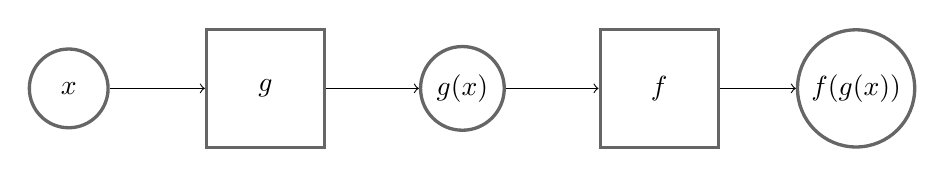
\begin{tikzpicture}[
roundnode/.style={circle, draw=black!60, fill=white!5, very thick, minimum size=10mm},
squarednode/.style={rectangle, draw=black!60, fill=white!5, very thick, minimum size=15mm},
]
    \node[roundnode] (x) {\(x\)};
    \node[squarednode] (maintopic) [right of=x, xshift=1.5cm] {\(g\)};
    \node[roundnode] (fx) [right of=maintopic, xshift=1.5cm] {\(g(x)\)};
    \node[squarednode] (gtopic) [right of=fx, xshift=1.5cm] {\(f\)};
    \node[roundnode] (final) [right of=gtopic, xshift=1.5cm] {\(f(g(x))\)};
    \draw[->] (maintopic.east) -- (fx.west);
    \draw[->] (x.east) -- (maintopic.west);
    \draw[->] (fx.east) -- (gtopic.west);
    \draw[->] (gtopic.east) -- (final.west);
  \end{tikzpicture}
  \caption{Visual representation of function composition.}

\end{figure} 

Another notation for composing functions together(which we will not really use) is as such:
\begin{equation*}
  f(g(x))=(f \circ g)(x) 
\end{equation*}

When you compose the same function \(n\)-times, the notation for it is:
\begin{equation*}
f^n(x)=\underbrace{f(f(\ldots f(x)))}_{n-times} 
\marginnote{\footnotesize \textit{However, this does not \\ apply to trigonometric functions. \(sin^2(x)\) is \(sin(x) \times sin(x)\) instead of \(sin(sin(x))\) and \(sin^{-1}(x)\) is \(arcsin(x)\).}}
\end{equation*}
\newpage
\begin{example}
  Here are some examples of composing functions together:
  If \(x=3\) and \(f(x)=\pi x\), \(g(x)=sin(x)+1\):
  \begin{equation}
    g(f(x))=sin(\pi \times 3)+1=1 
  \end{equation}
  \begin{equation}
    f^3(x)=\pi^{3}x 
  \end{equation}
  \quad \, There is nothing much here, really, just evaluate the function from the innermost function to the outermost.
\end{example}
\begin{theorem}
  Given functions \(f:X \to Y\), \(g: Y \to Z\) and \(h: Z \to W\), prove that the composition of the three functions is \textit{associative}, in other words:
  \begin{equation*}
    h \circ (g \circ f) = (h \circ g) \circ f
  \end{equation*}
\end{theorem}
\begin{proof}
  Let \(x \in X\), we have: 
  \begin{equation*}
    h \circ (g \circ f(x)) = h(g \circ f(x)) = h(g(f(x))) = h \circ g(f(x)) = (h \circ g)f(x)
  \end{equation*}
  This proves the associativity of function composition.
\end{proof}
\begin{remark}
  This is just a fun little exercise for the reader and ultimately is not that important to the entire book, just a good identity to keep in the back of your mind. 
\end{remark}

Next, we will delve into inverse functions. Let us start with one I believe you may have seen before, look at the following figure: 
\begin{figure}[h]
  \centering
  \begin{tikzpicture}[scale=1.8]
        \coordinate (a) at (0,0);
        \coordinate (b) at (4,0);
        \coordinate (c) at (4,2);
        \draw (a) -- (b)node[midway, below]{a} -- (c)node[midway,right]{b} -- (a)node[midway,left, above]{c}; % Triangle.
        \draw (a) node[anchor=east,align=center] {B};
        \draw (b) node[anchor=west,align=center] {C};
        \draw (c) node[anchor=south]{A};
        \MarkRightAngle{a}{b}{c}; 
\end{tikzpicture}
\caption{Figure of right triangle ABC.}
\end{figure}

If I ask you what is \(arcsin(B)\), you may say it is \(\frac{b}{c}\). But, what is \(arcsin(sin(B))\), well, that is just \(B\), isn't it. Hence, the \(arcsin\) sort of "cancels" the \(sin\). We call \(arcsin\) the \textit{inverse function} or just inverse of \(sin\). 

 \end{document}
